\documentclass{article}

\usepackage{tikz}
\usepackage[compat=1.1.0]{tikz-feynman}
\usetikzlibrary{angles, quotes}
\usetikzlibrary{calc}
\usetikzlibrary{external}
\usetikzlibrary{decorations.pathreplacing, shapes.misc}
\tikzexternalize[prefix=tikz/]
\tikzset{external/system call={lualatex \tikzexternalcheckshellescape -halt-on-error -interaction=batchmode -jobname "\image" "\texsource"}}
\usepackage{shellesc}

\usepackage{currfile}
\usepackage{etoolbox}
\newcommand*\setmyname{%
  \expandafter\tikzsetfigurename\expandafter{\currfilebase-}%
}
\AtBeginEnvironment{tikzpicture}{\setmyname}

\usepackage[backend=biber, style=ieee]{biblatex}  
\addbibresource{biblio.bib}


\usepackage[english]{babel}
\usepackage[a4paper]{geometry}
\usepackage{pgfplots}
\pgfplotsset{compat=1.17} 
\usepgfplotslibrary{fillbetween}

\usepackage{array}
\usepackage{multirow}
\usepackage{enumitem}
\usepackage{tabularx}
\usepackage{amsmath}
\usepackage{amssymb}
\usepackage{amsfonts}
\usepackage{physics}
\usepackage{graphicx}
\usepackage[colorlinks=true, allcolors=blue]{hyperref}
\usepackage{dsfont}

\newcommand{\Ms}[0]{\textup{M}_\odot}

\let\ov\overline
\let\lra\leftrightarrow
\let\ra\rightarrow
\let\xra\xrightarrow
\let\la\leftarrow
\let\nl\newline
\let\mcl\mathcal
\let\up\uparrow
\let\dow\downarrow


\tikzset{
odot/.style={
  circle,
  inner sep=0pt,
  node contents={$\odot$},
  scale=0.8
},
otimes/.style={
  circle,
  inner sep=0pt,
  node contents={$\otimes$},
  scale=0.8
}}


\newcolumntype{C}{>{\centering\arraybackslash}X}

\title{Premier Rapport de stage de Recherche au LPNHE\\\vspace{.3em} \large Mesure de la croissance des structures avec les galaxies du DESI BGS et les supernovae de type Ia de ZTF~: vers une analyse jointe}
\author{Antoine Gilles--Lordet\\ \vspace{.1em} \small encadré par Pauline Zarrouk et Nicolas Regnault }
\date{}

\begin{document}

\maketitle

\section{Reformulation de la problématique}

%  La reformulation de la problématique : Votre sujet, inscrit sur la fiche de stage, a certainement évolué. Vous connaissez maintenant le contexte de votre stage, vous pouvez réaliser un diagnostic de la situation pour remettre en question les mots de votre problématique et la quantifier.

Le modèle cosmologique qui rend le mieux compte des observations actuelles est le modèle $\Lambda$CDM basé sur la Relativité Générale. Ce modèle introduit deux grandes inconnues que sont la matière noire froide (\textit{Cold Dark Matter}) et l'énergie noire (sous la forme d'une constante cosmologique $\Lambda$), 

Une des sondes cosmologiques utilisées pour contraindre ce modèle est l'analyse du \textit{galaxy clustering}. En étudiant la distribution spatiale des galaxies ainsi que leurs vitesses, on calcule le paramètre $f\sigma_8$ qui décrit la formation et la croissance des structures de matière dans l'univers ainsi que l'histoire de l'expansion de l'univers basée sur une théorie de la gravité. Comme ce paramètre est prédit par les modèles cosmologiques, cela permet de tester la validité de la Relativité Générale aux échelles connues. Cependant les analyses de \textit{clustering} actuelles n'offrent pas une précision suffisante à très bas redshift à cause de la variance cosmique~: le volume de notre univers proche est limité et on ne voit qu'une réalisation possible d'un univers, on ne peut donc pas facilement distinguer une variation significative de $f\sigma_8$ d'un bruit statistique.

\begin{figure}
    \centering
    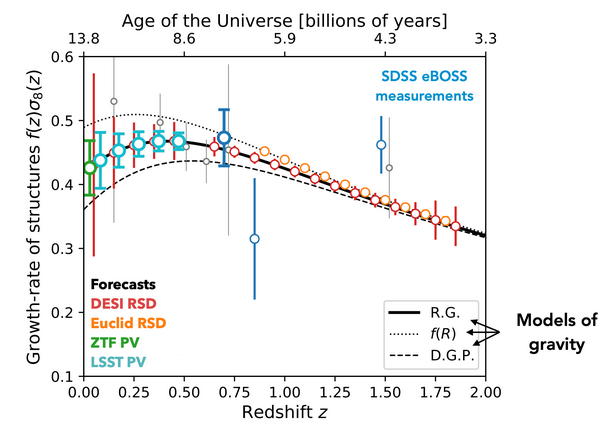
\includegraphics[width=0.8\textwidth]{figures/fs8.png}
    \caption{Prévisions des contraintes sur $f\sigma_8$ attendues de DESI, Euclid et de la combinaison de DESI avec ZTF PV ou LSST PV with DESI. Crédit~: J. Bautista}
    \label{fig:fs8}
\end{figure}

On dispose également d'une deuxième sonde à bas redshift, les observations de SuperNovae (SNe) de type Ia. Ces SNe sont des explosions thermonucléaire de naine blanche, riches en carbone et oxygène, et présentent la particularité d'être très similaires les unes aux autres. Grâce à cette standardisabilité, on peut produire des diagrammes de Hubble (magnitudes apparentes VS redshift) de ces SNe et obtenir ainsi des contraintes sur les paramètres cosmologiques. La réalisation de ce diagramme est actuellement l'objet du projet LEMAITRE au LPNHE, qui vise à développer un nouveau pipeline adapté au traitement des volumes de données attendus des prochains programmes d'observation. Une fois la standardisation effectuée et le modèle accordé au diagramme de Hubble, les résidus au modèle donnent accès aux vitesses particulières des SNe, c'est-à-dire la vitesse des galaxies hôtes des SNe par rapport à l'expansion de l'univers. Cet effet est représenté en Fig. \ref{fig:residues}, si les hôtes des SNe n'avaient pas de vitesses particulières, le redshift des SNe proviendrait uniquement de l'expansion de l'univers et elles s'aligneraient parfaitement sur le modèle. En réalité, elles sont décalées horizontalement par rapport à la ligne de base du modèle car les vitesses particulières de leurs hôtes est la source d'un effet Doppler additionnel qui modifie leur redshift : les SNe qui se rapprochent de nous apparaissent plus bleues et celles qui s'éloignent de nous apparaissent plus rouges qu'elles ne devraient l'être. On peut donc également remonter à des positions (via leurs positions dans le ciel et leurs redshifts) et des vitesses particulières (via leurs résidus au diagramme de Hubble), et en tirer une analyse $f\sigma_8$.


La combinaison de ces deux analyses doit donc permettre de mieux décrire les contraintes existantes à bas redshift. En Figure \ref{fig:fs8}, issue de \cite{carreres_growth-rate_2023}, est représenté les prévisions des contraintes sur $f\sigma_8$ en fonction du redshift pour différents relevés : les points expériementaux de SDSS et eBOSS en bleu, les prévisions de DESI et Euclid, et les prévisions de la combinaison de DESI avec les vitesses particulières issues des SNe de ZTF ou du futur relevé de SNe LSST. Le trait plein est la courbe théorique obtenue à partir de la Relativité Générale et ceux en pointillés représentent d'autres modèles de gravité. Les données de DESI seules ne permettent pas de discrimner différents modèles à bas redshift du fait de la taille des barres d'erreurs, alors qu'introduire les vitesses particulières issues de SNe les réduit grandement pourrait permettre une telle discrimination.

\begin{figure}
    \centering
    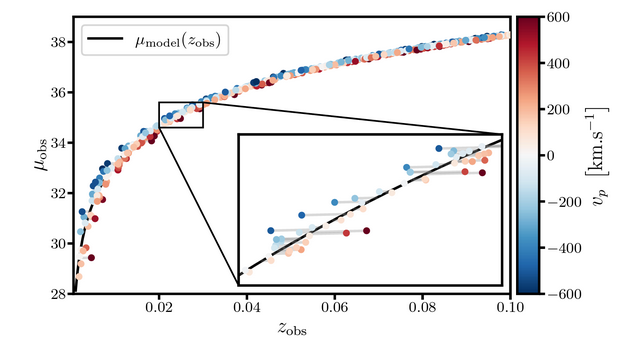
\includegraphics[width=0.8\textwidth]{figures/Residues.png}
    \caption{Résidus de SNe simulées au diagramme de Hubble. Crédit : B. Carreres}
    \label{fig:residues}
\end{figure}

Pour ce stage je travaille sur le relevé \textit{DESI Bright Galaxy Survey} (BGS) qui est un set complet de galaxies lumineuses ($r < 19.5$ pour le sous-échantillon \textit{Bright}) à bas redshift ($z<0.4$) \cite{hahn_desi_2023}. Plus particulièrement, j'utilise les données d'une simulation de matière noire à N-corps nommée Uchuu \cite{prada_desi_2023}, qui est peuplée avec des galaxies BGS pour produire un univers fidèle statistiquement au notre. Concernant les supernovae, j'exploite le relevé de SNe Ia à $z<0.1$ issu du programme de suivi des évènements transitoires \textit{Zwicky Transient Facility} (ZTF) \cite{bellm_zwicky_2018}.

\section{Mission}

%  L’appropriation de la mission : Y-a-t-il un repositionnement important des missions ? Si oui, quelle est votre nouvelle lettre de mission ? Quels sont les livrables que vous devrez rendre à la fin de votre stage ?

L'objectif du stage est double~:
\begin{enumerate}
    \item Produire des échantillons simulés de SNe basés sur les positions des galaxies de la simulation Uchuu qui reproduit les données spectroscopiques du DESI BGS, ainsi que les observations de ZTF, et les utiliser pour tester le pipeline LEMAITRE actuellement en développement au LPNHE pour produire les diagrammes de Hubble et reconstruire la cosmologie sous-jacente des échantillons.
    \item Comparer les résultats de ce pipeline, \textit{i.e.} les positions ainsi que les vitesses particulières reconstruites, aux données d'entrée et les utiliser pour
    	\begin{enumerate}
		\item Estimer $f \sigma_8$ à partir des vitesses particulières de SNe de ZTF et comparer ces résultats avec ceux de B. Carreres \cite{carreres_growth-rate_2023}.
		\item Produire une analyse jointe du DESI BGS et des SNe de ZTF pour quantifier le gain sur les contraintes de $f\sigma_8$.
	\end{enumerate}
\end{enumerate}

À l'issu du stage, un rapport technique sur le travail effectué ainsi que le code produit sera rendu aux membres du groupe cosmologie du LPNHE. Ce rapport décrira les méthodes suivies, les approximations éventuelles et les paramètres de simulation utilisés afin de permettre à d'autres membres de réutiliser le code à d'autres fins. Le code produit lors du stage devra donc également s'interfacer facilement avec les outils existants et ceux actuellement en développement.

\section{Enjeux}

%  les enjeux pour l’entreprise et les résultats tangibles attendus de vous à l'issue du stage sur votre (vos) différente(s) mission(s) en distinguant clairement les niveaux équipe et individuel

L'enjeu principal pour le pipeline LEMAITRE est la production d'un échantillon simulé dont les caractéristiques sont différentes des échantillons habituels. Cet échantillon peut servir à diagnostiquer des biais potentiels dans l'analyse, et tester les différentes étapes du pipeline dans des conditions réalistes. Un deuxième enjeu est que la conduite d'une analyse $f\sigma_8$ sur des données de SNe à bas redshift en utilisant le pipeline LEMAITRE permettra de comparer les résultats obtenus aux études existantes ainsi que les performances de ce pipeline en matière d'inférence cosmologique.

Au niveau individuel, l'enjeu est de développer des compétences en analyse de données de SNe Ia, en inférence de paramètres cosmologiques à partir d'observations, ainsi qu'en simulations cosmologiques.

\section{Planning}

%  le planning « grosses mailles » de votre mission faisant apparaître les grandes étapes et en particulier les points de décision où vous aurez à communiquer vers des décideurs

Comme ce projet faisait déjà l'objet de mon projet de mention, le premier objectif est déjà bien entamé. Dans l'idéal il sera fini au plus tard fin mai, puis je me focaliserai sur l'analyse $f\sigma_8$ jusqu'à la fin du stage. L'analyse des SNe de ZTF devrait durer jusqu'à fin juillet, puis je tenterai de produire une analyse jointe DESI/ZTF. Si ces analyses sont finalisées plus tôt, la rédaction d'un article pourra être envisagée, ainsi que de contribuer plus directement au développement du pipeline LEMAITRE.

\section{Feedback}

%  le processus de feedback et d'évaluation prévu vous concernant personnellement et sa périodicité

Comme le stage s'effectue en parallèle du développement du pipeline LEMAITRE, j'assiste aux réunions hebdomadaires pour suivre l'avancement des différents outils qui le compose, en particulier celles sur lesquelles mon code s'interface. A ces réunions s'ajoutent des points réguliers avec mes encadrants, Pauline Zarrouk et Nicolas Regnault, à raison d'au moins une fois par semaine pour partager mon avancement ou résoudre d'éventuels problèmes.

% Par ailleurs je vais également présenter mes travaux au groue de travail ``Low-z and transients'' de DESI et participer à la réunion annuelle de la collaboration en juillet à Marseilles.

\printbibliography


\end{document}
